% Describe the test setup to verify that your problems from 1.3 have been solved.
% This can be done in different ways depending on focus of your problems.
% Some problems may purely objective, such as "improve the performance of X compared to Y".
% These are easy to evaluate since you simply need to compare the performance, and perhaps compare against a few more technologies that you have listed in Section 2 (related work).
% In other cases the problems may be very subjective, such as "Create a mobile app that can be used while driving, and which shows the most fuel efficient time to change gear".
% This problem will require a user-study in which several persons drive without the application, you calculate the fuel consumption, then they drive with the application and then you calculate the fuel consumption again.
% Then you collect the objective measurements (fuel consumption comparisons) and the subjective opinions from the users about whether the application was unobtrusive, usable, etc. (typically via a questionnaire).



% New Result Tables

%\begin{table}[h]
%	\centering
%	\small
%	\begin{tabular}{ |p{2cm}|p{8cm}|  }
%		\hline
%		\multicolumn{2}{|c|}{\textbf{The debuggers evaluation results for variable \emph{test\_enum3}}} \\ 
%		\hline
%		\hline
%		Source & Value \\
%		\hline
%		\glsfull{pc} & 0x08000604 \\
%
%		DWARF Locaiton & (DW_OP_piece: 9; DW_OP_breg13 (r13): 156; DW_OP_piece: 3) \\
%
%		Rust Source Code & let mut test\_enum3 = TestEnum::Struct(TestStruct \{ flag: true, num: 123\}); \\
%		\hline
%		\hline
%		Debugger (Version) & Evaluated Result \\
%		\hline
%		ERD (0.1.0) & test\_enum3 = TestEnum \{ \textless \ OptimizedOut \textgreater \} \\
%TestEnum { < Variant > = < OptimizedOut >, 0 { ITest = ITest { __0 = < OptimizedOut >, }, }, 1 { UTest = UTest { __0 = < OptimizedOut >, }, }, 2 { Struct = Struct { __0 = TestStruct { num = < OptimizedOut >, flag = < OptimizedOut >, }, }, }, 3 { Non = Non, }, }
%
%		GDB (11.0.90)  & (gdb) p test\_enum3\newline
%		\$ 1 = nucleo\_rtic\_blinking\_led::TestEnum::ITest(\newline
%		\textless optimized out\textgreater) \\
%
%		LLDB (13.0.0) & (nucleo\_rtic\_blinking\_led::TestEnum) test\_enum3 = \{\newline
%		\text{\ \ ITest = (0 = 0)}\newline
%		\text{\ \ UTest = (0 = 0)}\newline
%		\text{\ \ Struct = \{}\newline
%		\text{\ \ \ \ 0 = (flag = false, num = 0)}\newline
%		\text{\ \ \}}\newline
%		\text{\ \ Non = \{\}}\newline
%		\} \\
%		\hline
%	\end{tabular}
%	\label{table:enum3}
%	\caption{The different debuggers evaluation result for variable \emph{test\_enum3}, and the actual soruce code value and DWARF location.}
%\end{table}
%
%
%\begin{table}[h]
%	\centering
%	\small
%	\begin{tabular}{ |p{2cm}|p{8cm}|  }
%		\hline
%		\multicolumn{2}{|c|}{\textbf{The debuggers evaluation results for variable \emph{test\_struct}}} \\ 
%		\hline
%		\hline
%		Source & Value \\
%		\hline
%		\glsfull{pc} & TODO \\
%
%		DWARF Location & (DW_OP_breg13 (r13): 260) \\
%
%		Rust Source Code & let mut test\_struct = TestStruct \{ flag: true, num: 123 \}; \\
%		\hline
%		\hline
%		Debugger (Version) & Evaluated Result \\
%		\hline
%		ERD (0.1.0) & test\_struct = TestStruct \{ num::123, flag::\textless \ OptimizedOut \textgreater \} \\
%
%		GDB (11.0.90)  & (gdb) p test\_struct\newline
%		\$ 1 = nucleo\_rtic\_blinking\_led::TestStruct \{flag: \textless synthetic pointer\textgreater, num: 123\} \\
%
%		LLDB (13.0.0) & (nucleo\_rtic\_blinking\_led::TestEnum) test\_struct = (flag = false, num = 123) \\
%		\hline
%	\end{tabular}
%	\label{table:struct}
%	\caption{The different debuggers evaluation result for variable \emph{test\_struct}, and the actual soruce code value and DWARF location.}
%\end{table}
%
%
%\begin{table}[h]
%	\centering
%	\small
%	\begin{tabular}{ |p{2cm}|p{8cm}|  }
%		\hline
%		\multicolumn{2}{|c|}{\textbf{The debuggers evaluation results for variable \emph{test\_array}}} \\ 
%		\hline
%		\hline
%		Source & Value \\
%		\hline
%		\glsfull{pc} & 0x08000604 \\
%
%		DWARF Location List Ranges & 000003fc ffffffff 080002b8
%    00000404 080002f2 0800038e\newline 
%    0000042d 0800038e 080003ee\newline
%    00000455 0800048a 080005cc\newline
%    000004cf 080005cc 080005ce\newline
%    0000053e 080005ce 080005d0\newline
%    000005ae 080005d0 080005d2\newline
%    00000613 080005d2 080005d4\newline
%    00000679 080005d4 080005d6\newline
%    000006d4 080005d6 080005d8\newline
%    00000730 080005d8 080005da\newline
%    00000781 080005da 080005dc\newline
%    000007d3 080005dc 080005de\newline
%    0000081a 080005de 080005e0\newline
%    00000862 080005e0 080005e2\newline
%    0000089f 080005e2 080005e4\newline
%    000008dd 080005e4 080005e6\newline
%    00000910 080005e6 080005ee\newline
%    00000944 080005ee 0800067a\newline 
%    0000096d 08000688 08000694\newline\\
%
%		Rust Source Code & let mut test\_array = [-12, 8]; \\
%		\hline
%		\hline
%		Debugger (Version) & Evaluated Result \\
%		\hline
%		ERD (0.1.0) & test\_array = \textless LocationOutOfRange\textgreater \\
%
%		GDB (11.0.90)  & (gdb) p test\_array\newline
%		\$ 3 = \textless optimized out\textgreater \\
%
%		LLDB (13.0.0) & TODO \\
%		\hline
%	\end{tabular}
%	\label{table:array}
%	\caption{The different debuggers evaluation result for variable \emph{test\_array}, and the actual soruce code value and DWARF location.}
%\end{table}


%

% Move to above section

The testing and comparing of the three different debuggers is done manually on some example code, see the git repository \cite{example-code} for the example code.
The example code was many times modified to test how well the three debugger handled the different situations.
This was repeated until one of the debuggers gave an unexpected result.
There were two of these cases found when the code was compiled with optimization 2.
To keep it fair in these cases a software breakpoint was added to the code.
This ensures that all the three debuggers stops on the same machine code instruction.
The reason being that the debug result can be correct but still different from the other debugger, thus making it seem like one is worse then the other.


\subsubsection{Evaluation of \emph{Rust} enums}
The \emph{GDB} debugger gave the wrong value when debugging the value of a enum named \emph{test\_enum3}, the result can be seen in figure \ref{fig:gdbenum}.
The expected value is \emph{TestEnum::Struct(TestStruct { flag: true, num: 123 })} which is not the same as what \emph{GDB} gave.


\begin{figure}[h]
	\centering
	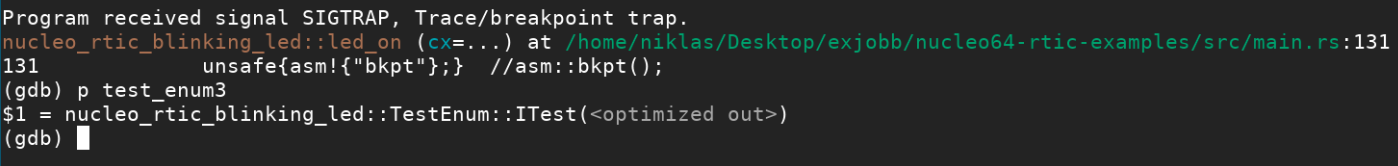
\includegraphics[width=0.9\textwidth]{gdb10.1-opt2-enum-edited.png}
	\caption{\emph{GDB} debugging result from evaluating variable \emph{test\_enum3} when stopped at the software breakpoint in the example code.}
	\label{fig:gdbenum}
\end{figure}


Doing the same using \gls{erd} also gives an unexpected value, the result can be seen in  figure \ref{fig:mydebuggerenum}.
The printing look a bit different but the result from the \gls{erd} debugger tells the user that the enum \emph{test\_enum3} is an enum of type \emph{TestEnum} where the actual variant has been optimized out.
While \emph{GDB} also tells that \emph{test\_enum3} is of type \emph{TestEnum}, but it also shows that the enum variant is \emph{ITest}.
As can be observed in figure \ref{fig:gdbenum}, \emph{GDB} gives the wrong answer because it says that \emph{test\_enum3} is the enum variant \emph{TestEnum::ITest} which is wrong.
While the \gls{erd} debugger shows that the value has been optimized out which is a more proper response in this case.


\begin{figure}[h]
	\centering
	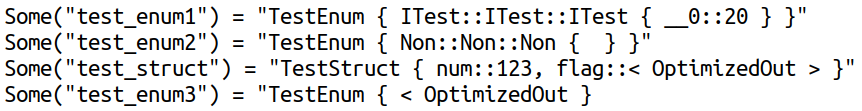
\includegraphics[width=0.9\textwidth]{my-debugger-opt2-enum-edited.png}
	\caption{\acrshort{erd} debugging result from evaluating some enum variables when stopped at the software breakpoint in the example code.}
	\label{fig:mydebuggerenum}
\end{figure}


Doing the same using \emph{LLDB} give almost the same result as \gls{erd}, that result can be seen in figure \ref{fig:lldbenum}.
\emph{LLDB} does not show that the variant of the enum has been optimized out which makes the reason why it is not printed ambiguous.


\begin{figure}[h]
	\centering
	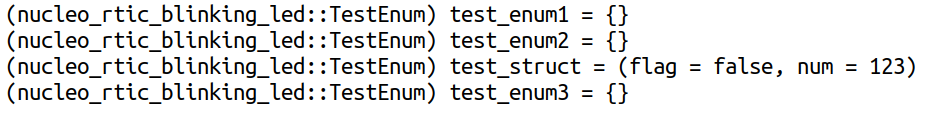
\includegraphics[width=0.9\textwidth]{lldb11.0-opt2-enum-edited.png}
	\caption{\emph{LLDB} debugging result from evaluating some enum variables when stopped at the software breakpoint in the example code.}
	\label{fig:lldbenum}
\end{figure}


Now when inspecting what is stored in the \gls{DWARF} format it shows that the variant of the enum is optimized out but not the two other values that make up the value stored in the variant.
The fact that the value indicating the variant type is optimized out makes it impossible for any debugger to evaluate the value stored in the enum.
This is because the encoding of the bytes is unknown and because the number of bytes to read from the stack is unknown.


Looking back at figure \ref{fig:lldbenum} there are three other enums where two of them do not have a value.
They are named \emph{test\_enum1} and \emph{test\_enum2}.
Those two enums should have a value but for some reason \emph{LLDB} is not able to evaluate them.
However the debugger \gls{erd} is able to the correct value of them, see figure \ref{fig:mydebuggerenum}.
Also looking at figure \ref{fig:gdbenum} shows the same result as in figure \ref{fig:mydebuggerenum} thus both \emph{GDB} and \gls{erd} is able to evaluate the correct value.


Going back again to figure \ref{fig:lldbenum} which shows that the value of the attribute \emph{flag} is equal to \emph{false}, but looking at figure \ref{fig:gdbenum} and \ref{fig:lldbenum} shows that the value of \emph{flag} is equal to \emph{true}.
The correct value when looking at the original source code is that the attribute \emph{flag} should be equal to \emph{true}, thus meaning that the result from \emph{LLDB} is incorrect.



\subsubsection{Displaying Optimized Out Variables}
Another problem found is with values that are temporarily not present in any register or the stack which means that it is temporarily optimized out or out of range.
An example of this is the value of the variable \emph{test\_u16} which is a unsigned $16$ bit integer that is temporarily optimized out when stopped at the software breakpoint in the example.
When evaluating this value \emph{GDB} prints that the value is optimized out which can be seen in figure \ref{fig:gdboutofrange}, this is the same output it gives for a value that is totally optimized out(example of this is the value of \emph{test\_struct} shown in figure \ref{fig:gdbenum}).


\begin{figure}[h]
	\centering
	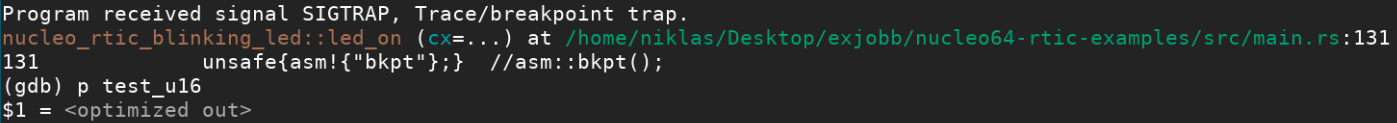
\includegraphics[width=0.4\textwidth]{gdb10.1-opt2-outofrange-edited.png}
	\caption{\emph{GDB} debugging result from evaluating variable \emph{test\_u16} when stopped at the software breakpoint in the example code.}
	\label{fig:gdboutofrange}
\end{figure}


Doing this with \emph{LLDB} gives the result  \emph{$<$ variable is not available $>$} which can be seen in figure \ref{fig:lldboutofrange}.


\begin{figure}[h]
	\centering
	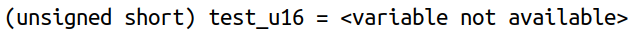
\includegraphics[width=0.9\textwidth]{lldb11.0-opt2-outofrange-edited.png}
	\caption{\emph{LLDB} debugging result from evaluating variable \emph{test\_u16} when stopped at the software breakpoint in the example code.}
	\label{fig:lldboutofrange}
\end{figure}


Lastly comparing this to the output of \gls{erd}, which give the value \emph{$<$OutOfRange$>$}, see figure \ref{fig:mydebuggeroutofrange}.
The result from both \emph{LLDB} and \gls{erd} are unique and only happen in these situations thus making it easier for the user to understand that the value is temporary optimized out than the result from \emph{GDB}.
This is because the result that \emph{GDB} generates is used in multiple situations thus making it unclear if the variable is totally optimized out or temporarily optimized out.


\begin{figure}[h]
	\centering
	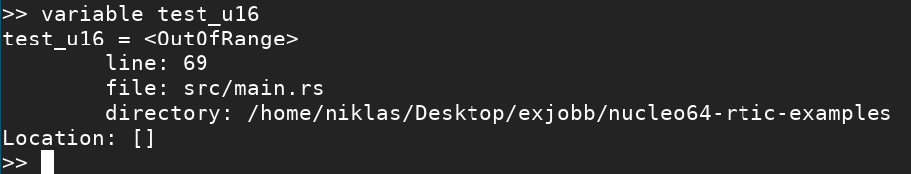
\includegraphics[width=0.9\textwidth]{my-debugger-opt2-outofrange-edited.png}
	\caption{\gls{erd} debugging result from evaluating variable \emph{test\_u16} when stopped at the software breakpoint in the example code.}
	\label{fig:mydebuggeroutofrange}
\end{figure}

